\documentclass{beamer}
\usepackage{stackengine}
\usepackage{mathtools}
\renewcommand\useanchorwidth{T}
\usepackage{xcolor}
\def\theyearwidth{1.5pt}
\def\mystrut{\rule{0ex}{.1ex}}
\def\myyrstrut{\rule[-1ex]{0ex}{2ex}}
\newlength\yrsfboxrule
\yrsfboxrule .4\fboxrule
\newcommand\yearwidth[1]{\def\theyearwidth{#1}\ignorespaces}
\newcommand\skipyears[2][black]{%
  \fboxrule\yrsfboxrule%
  \fboxsep=-\yrsfboxrule%
  \fcolorbox{#1}{#1}{\mystrut\hspace{#2}}%
  \ignorespaces%
}
\newcommand\showyear[2][black]{%
  \fboxsep=0pt%
  \stackunder[2pt]{%
    \colorbox{#1}{\myyrstrut\hspace{\theyearwidth}}%
  }{\tiny#2}%
  \ignorespaces%
}
\usetheme{Amsterdam}

\title{Approximation Algorithms for Stochastic Inventory Control Models}
\subtitle{A periodic-review stochastic inventory control problem}
\author[Hao Yuan, Feng Wei, Blake Miller]{Hao Yuan, Feng Wei, Blake Miller  {\ttfamily Github:\href{https://github.com/blakeapm/stochastic-inventory}{github.com/blakeapm/stochastic-inventory}}}
\date{\today}

\begin{document}
  \frame{\titlepage}
  \section{The Periodic-Review Stochastic Inventory Control Problem}
  \subsection{General Concepts}
  \begin{frame}
    \frametitle{The Periodic-Review Stochastic Inventory Control Problem}
    \begin{itemize}
      \item Computing a provably efficient inventory control policies is difficult because:
        \begin{itemize}
          \item demand per time-period is correlated
          \item demand is non-stationary (time-dependent, distribution changes with time)
          \item cost is hard to predict due to the nature of demand
        \end{itemize}
      \item Important for any company that seeks to minimize cost of holding excess inventory while minimizing backorder costs (unmet demand)
      \item Particularly important in industries where the demand environment is highly dynamic. (i.e. Apple's supply-chain for solid state drives, seasonal products such as rock salt)
      \item These environments experience high correlation between demands in different periods (difficult to compute optimal inventory policy).
    \end{itemize}
  \end{frame}
  \subsection{Minimizing Cost}
  \begin{frame}
    \frametitle{Minimizing Expected Cost}
    Our goal is to supply each unit of demand without ordering too early or too late. This is difficult because:
    \begin{itemize}
      \item Oftentimes demand and lead times (time between order and receipt of product) are unpredictable.
      \item Inaccuracies can be extremely costly, so it is important that approximations are provably accurate within a certain range of error
    \end{itemize}
    To illustrate the problem, a different, and simpler algorithm:
      \begin{center}
      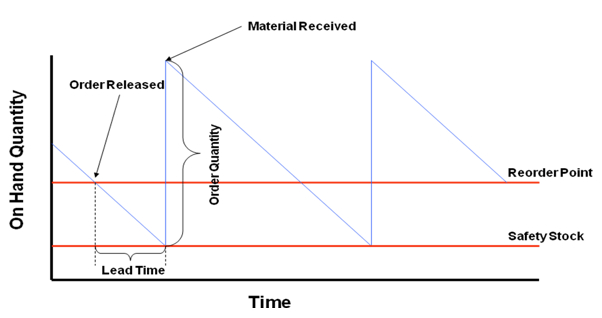
\includegraphics[height=1.5in]{purchasing.png}
      \end{center}
  \end{frame}

  \section{Expected Cost Function}
  \subsection{Minimizing Expected Cost}
  \begin{frame}
    \frametitle{Model}
    We consider finite time horizon $T$.
    \par
      {\centering\yearwidth{1pt}\tclap{\tiny t}\showyear{1}\skipyears[black]{.5in}\showyear{2}\skipyears[black]{.5in}\showyear{3}\skipyears[black]{.5in}\showyear{4}\skipyears[black]{.5in}\showyear{5}\skipyears[black]{.5in}\showyear{6}\skipyears[black]{.5in}$\text{  }\cdots\text{  }$\showyear{$T-1$}\skipyears[black]{.5in}\showyear{$T$}
    \par}
    \vspace{0.1in}
    At each time period $t = 1,\cdots,T$, the following cost are incurred
        \[L_t(x_t,d_t,q_t):=c_tq_t+h_t(x_t + q_t - d_t)^{+}+p_t(x_t + q_t -d_t)_{t}^{-}\]
        (Local Cost = Ordering Cost + Holding Cost + Backloging Cost)
    \begin{itemize}
      \item $c_t$: per-unit ordering cost at time $t$.
      \item $h_t$: per-unit holding cost from $t$ to $t + 1$.
      \item $p_t$: per-unit backlogging penalty at time $t$.
      \item $x_t$: net inventory at time $t$. (our state)
      \item $q_t$: ordering quantity at time $t$. (our control)
      \item $d_t$: demand quantity at time $t$. (we observe $d_t$ after decide $q_t$)
    \end{itemize}
  \end{frame}

  \begin{frame}
    Goal: At time $t$, choose $q_t$ to minimize the expected total cost from period $t$ to $T$.\\
    Let $V_t$ be the minimum expected cost from period $t$ to $T$. Then
    \begin{eqnarray*}
    V_T(x_T,d_{1..T-1}) =& \min_{q_T \geq 0} E[L_T(x_T,D_T,q_T) | d_{1..T-1}]\\
    V_t(x_t,d_{1..t-1}) =& \min_{q_t \geq 0} E[L_t(x_t,D_t,q_t)\\
                        &+V_{t+1}(x_t + q_t - D_t, d_{1..t-1},D_t)|d_{1..t-1}]
    \end{eqnarray*}
    
    This gives us two natural ways to "solve" the problem:
    \begin{itemize}
      \item 
        Dynamic Programming: solve for $q_t$ backwards using the formula above.
      \item
        Myopic: At time $t$, ignore $V_{t+1}$, we only minimize $E[L_t(x_t,D_t,q_t)|d_{1..t-1}]$.
    \end{itemize}

  \end{frame}

\begin{frame}
Recall: 
    \begin{eqnarray*}
    V_T(x_T,d_{1..T-1}) =& \min_{q_T \geq 0} E[L_T(x_T,D_T,q_T) | d_{1..T-1}]\\
    V_t(x_t,d_{1..t-1}) =& \min_{q_t \geq 0} E[L_t(x_t,D_t,q_t)\\
                        &+V_{t+1}(x_t + q_t - D_t, d_{1..t-1},D_t)|d_{1..t-1}]
    \end{eqnarray*}
    \begin{itemize}
      \item 
        At period $s>t$, $D_s$ is a random variable that depends on perivous demands $d_1, d_2,...,d_{t+1},...,d_{s-1}$.\\
        To compute the above conditional expectation, we need to work on $q_t,...,q_T$ which are are our future decision.\\
      \item
        Myopic approach works extremly good on many cases, but may perform extremly bad on some cases. (Bad case example will be shown at the end of the talk.)
    \end{itemize}
\end{frame}


\begin{frame}
    \begin{itemize}
      \item 
        In fact we also need to consider leading time $L \neq 0$ (i.e. it takes $L$ periods to receive our order.) Then we need to modify:
        \begin{eqnarray*}
          x_t & := Net~Inventory + Undelived~orders\\
              & := Net~Inventory + \sum_{j = t - L+1}^{t-1} q_j\\
          L_t(x_t,d_{t..t+L},q_t)& :=c_tq_t + h_{t+L}(x_t + q_t - \sum d_{t..t+L})^{+} \\ 
                                &  + p_{t+L}(x_t + q_T - \sum d_{t..t+L})^{-}
        \end{eqnarray*}
        ***$ \sum d_{t..t+L} := d_t + ... + d_{t+L}$\\
        %***$Undelived~orders := \sum_{j = t - L+1}^{t-1} q_j$
      \item
        We can assume $c_t = 0$ by doing the transformation:
        \begin{eqnarray*}
          &\hat{c_t} := 0;\\
          &\hat{h_t} := h_t + c_t - c_{t+1}\\
          &\hat{p_t} := p_t - c_t + c_{t+1}
        \end{eqnarray*}
        ***$c_{T+1} := 0$
      \end{itemize}
\end{frame}


\begin{frame}
    \frametitle{Dual-Balancing Algotrithm}
    Recall {\em Local Backlogging Cost}: 
    $$\Pi_t(x_t,q_t) := p_{t+L}(x_t + q_T - \sum D_{t..t+L})^{-}$$
    Now, we define {\em Marginal Holding Cost}:
    $$H_t(x_t,q_t) := \sum_{j = t+L}^{T} h_j (q_t - (\sum D_{t..j} - x_t)^+)^+$$.
    Dual-Balancing Algorithm:
    \begin{itemize}
      \item 
        Do transformation make ordering cost 0.
      \item
        Solve the convex optimaztion problem 
        $$q_t = argmin \max{E[H_t(x_t,q_t)| d_{1..t-1}], E[\Pi_t(x_t,q_t)| d_{1..t-1}]}$$
        in order to find out $q_t$ such that
        $$E[H_t(x_t,q_t)| d_{1..t-1}] = E[\Pi_t(x_t,q_t)| d_{1..t-1}]$$
    \end{itemize}
\end{frame}

\begin{frame}
    \frametitle{Coding and Chanllenge}    
    
\end{frame}

\begin{frame}
    \frametitle{Chanllenge in the Project}    
    
\end{frame}


  \section{The Algorithm and Computational Approaches}
    \subsection{Dynamic Programming}
    \begin{frame}
    \frametitle{Dynamic Programming}
      \begin{itemize}
        \item Let $V_{t}\left(x_{t}\right)$ be the optimal expected cost over over periods $t=t,\cdots,T.$
        \item Using dynamic programming, we can solve each $V_{t}$
        \item This approach would be accurate if it were feasible, but the term $E\left[V_{t+1}\left(x_{t}+q_{t}-D_{t}\right)\right]$ is very difficult to compute.
      \end{itemize}
    \end{frame}

    \subsection{Myopic (Na{\"i}ve) Approach}
    \begin{frame}
    \frametitle{Myopic (Na{\"i}ve) Approach}
      The myopic approach focuses only on minimizing the expected immediate cost that is going to be incurred in each period, while ignoring the cost over the rest of the horizon.
      \[c_{t}\left(q_{t}\right)+E\left[h_{t}\left(x_{t}+q_{t}-D_{t}\right)^{+}+p_{t}\left(x_{t}+q_{t}-D_{t}\right)^{-}\right]\]
    \end{frame}




    \subsection{Dual-Balancing Problem}
    \begin{frame}
    \frametitle{Dual-Balancing Problem}
      \[H_t^B(Q_t):=\sum\limits_{j=t+L}^T h_j(Q_t-(D_{[t,j]}-X_t)^+)^+\]
      \[\Pi_t^B:=p_t(D_{[t,t+L]}-(X_t^B+Q_t))^+=p_t(D_{[t,t+L]}-Y_t^B)^+\]
    \end{frame}

    \subsection{Why Dual-Balancing?}
    \begin{frame}
    \frametitle{Why Dual-Balancing?}

    \end{frame}
  \section{Coding and Implementation}
    \subsection{Coding and Implementation}
    \begin{frame}
    \frametitle{Coding and Implementation}

    \end{frame}
  \section{Results}
    \subsection{Time Complexity}
    \begin{frame}
    \frametitle{Time Complexity}
    Dual-balancing
    Myopic
    Dynamic Programming
    \end{frame}
    \subsection{Accuracy}
    \begin{frame}
    \frametitle{Accuracy}
    Dual-balancing vs. Myopic
    Dual-balancing vs. Dynamic Programming
    \end{frame}
  \section{Open Problems and Challenges in the Field of Stochastic Inventory Control}
    \subsection{Open Problems and Challenges in the Field of Stochastic Inventory Control}
    \begin{frame}
    \frametitle{Open Problems and Challenges in the Field of Stochastic Inventory Control}

    \end{frame}

\end{document}